\section{Filosofía operacional}
\label{inicio_cap3}

Skyfilms S.A.S. desarrolla operaciones con Sistemas de Aeronaves No Tripuladas (UAS) bajo un modelo de gestión orientado a la seguridad operacional, la estandarización de procedimientos y la mejora continua.

Todas las operaciones son planificadas, ejecutadas y supervisadas conforme a los requisitos establecidos en el Reglamento Aeronáutico de Colombia (RAC 100), las Especificaciones Operacionales (OpSpecs), el presente Manual de Operaciones, el Sistema de Gestión de la Seguridad Operacional (SMS) y el Manual de Control de Mantenimiento (MCM).

La seguridad operacional constituye el principio rector de todas las actividades desarrolladas por Skyfilms. En consecuencia, ninguna misión tendrá prioridad sobre la protección de las personas, la preservación de los bienes, el cumplimiento de la reglamentación aeronáutica o la integridad de las aeronaves y equipos utilizados.

\subsection{Principios operacionales}

Las operaciones desarrolladas por Skyfilms se fundamentan en los siguientes principios:

\begin{enumerate}[label=\arabic*.]

\item La seguridad operacional prevalece sobre cualquier objetivo comercial, operativo o contractual.

\item Ninguna operación será ejecutada sin una adecuada planificación y evaluación previa de los riesgos.

\item Toda misión deberá ser autorizada conforme a los procedimientos establecidos por la organización.

\item Todo el personal involucrado deberá conocer claramente sus funciones, responsabilidades y autoridad antes del inicio de la operación.

\item Las aeronaves únicamente serán utilizadas cuando se encuentren en condiciones técnicas adecuadas para la operación.

\item Todas las operaciones deberán generar registros documentales que permitan demostrar su planificación, ejecución y cierre.

\item Todo incidente, accidente o condición insegura será reportado y gestionado conforme al Sistema de Gestión de la Seguridad Operacional (SMS).

\item Skyfilms promoverá la mejora continua mediante el análisis de la información operacional, la retroalimentación del personal y la actualización permanente de sus procedimientos.
\end{enumerate}


\subsection{Objetivos operacionales}

Las operaciones UAS desarrolladas por Skyfilms tienen como objetivos principales:

\begin{itemize}

\item Garantizar operaciones seguras y conformes con la reglamentación aeronáutica.

\item Proteger la integridad de las personas, bienes y aeronaves.

\item Obtener productos audiovisuales de alta calidad para los clientes.

\item Mantener un elevado nivel de profesionalismo en todas las operaciones.

\item Fortalecer la cultura de seguridad operacional dentro de la organización.

\item Promover la mejora continua de los procesos operacionales.

\end{itemize}


\begin{tcolorbox}[title=Política Operacional de Skyfilms,colback=gray!5,colframe=black]

Skyfilms S.A.S. se compromete a desarrollar operaciones UAS bajo los más altos estándares de seguridad operacional, cumplimiento normativo y profesionalismo, promoviendo una cultura organizacional basada en la planificación, la gestión del riesgo, la disciplina operacional y la mejora continua.

Toda decisión operacional deberá orientarse a preservar la seguridad de las personas, proteger el espacio aéreo y garantizar la confianza de nuestros clientes y de la autoridad aeronáutica.

\end{tcolorbox}




\section{Flota UAS}
Skyfilms S.A.S. operará la siguiente flota, sujeta a los procesos de adquisición y registro formal ante la Aerocivil.

\subsection{Ficha Técnica: DJI Mavic 4 Pro}
\begin{table}[H]
    \centering
    \renewcommand{\arraystretch}{1.2}
    \begin{tabular}{|p{5cm}|p{9cm}|}
        \hline
        \rowcolor[gray]{0.9} \textbf{Parámetro} & \textbf{Especificación} \\ \hline
        \textbf{Marca / Modelo} & DJI / Mavic 4 Pro \\ \hline
        \textbf{Número de Serie / RUAS} & En proceso de adquisición \\ \hline
        \textbf{MTOW (Peso al despegue)} & 1085 g (MTOM según el Manual de usuario DJI Mavic 4 Pro, v1.0, p. 93) \\ \hline
        \textbf{Dimensiones} & 347 x 283 x 107 mm (desplegado) \\ \hline
        \textbf{Clasificación / Tipo de vuelo} & Multirrotor / VTOL (Despegue y aterrizaje vertical) \\ \hline
        \textbf{Velocidad máx. (Ascenso/Descenso/Vuelo)} & 8 m/s / 6 m/s / 21 m/s \\ \hline
        \textbf{Techo máx. de operación} & 6000 m s.n.m. \\ \hline
        \textbf{Autonomía / Radio de acción} & 43 minutos (sin viento); tiempo máximo de vuelo planificado: 80\,\% de la autonomía (RAC 100.210 k) / Hasta 750 m (Restricción VLOS) \\ \hline
        \textbf{Resistencia al viento / Temp.} & 12 m/s / -10°C a 40°C \\ \hline
        \textbf{Sistemas GNSS} & GPS + Galileo + BeiDou \\ \hline
        \textbf{Protección IP} & N/A \\ \hline
        \textbf{Frecuencias / Sistema C2} & 2.4 GHz y 5.8 GHz / DJI O4 (OcuSync 4) \\ \hline
        \textbf{Latencia / Encriptación} & Aprox. 120 ms / AES-256 \\ \hline
        \textbf{Detección de obstáculos} & Omnidireccional (APAS 5.0) \\ \hline
        \textbf{Carga útil / Cámara} & Sensor Hasselblad CMOS integrado \\ \hline
        \textbf{Fuente de energía} & Batería inteligente Li-ion \\ \hline
    \end{tabular}
\end{table}

\subsection{Ficha Técnica: BetaFPV Pavo20 Pro (FPV)}
\begin{table}[H]
    \centering
    \renewcommand{\arraystretch}{1.2}
    \begin{tabular}{|p{5cm}|p{9cm}|}
        \hline
        \rowcolor[gray]{0.9} \textbf{Parámetro} & \textbf{Especificación} \\ \hline
        \textbf{Marca / Modelo} & BetaFPV / Pavo20 Pro (cinewhoop FPV de 2,2 pulgadas) \\ \hline
        \textbf{Número de Serie / RUAS} & En proceso de adquisición (Serie de FC) \\ \hline
        \textbf{MTOW (Peso al despegue)} & Por pesar: aeronave lista para volar con batería, receptor y tira LED. Referencia del fabricante: 116 g sin batería, con transmisor DJI O4 Pro \\ \hline
        \textbf{Dimensiones} & Distancia entre ejes de 93,9 mm; hélices de 2,2 pulgadas de 3 palas. Medida D (con hélices): por medir, aprox. 0,15 m \\ \hline
        \textbf{Clasificación / Tipo de vuelo} & Multirrotor FPV / VTOL \\ \hline
        \textbf{Velocidad máx. (Ascenso/Descenso/Vuelo)} & Por determinar en vuelos de prueba (modo Acro) \\ \hline
        \textbf{Techo máx. de operación} & Por confirmar (límite operacional del manual: 400 ft AGL) \\ \hline
        \textbf{Autonomía / Radio de acción} & 8 a 10 min según batería (datos del fabricante con baterías 4S de 580 a 680 mAh); tiempo máximo de vuelo planificado: 80\,\% de la autonomía / Hasta 750 m (Restricción VLOS con observador) \\ \hline
        \textbf{Resistencia al viento / Temp.} & Por determinar en vuelos de prueba \\ \hline
        \textbf{Sistemas GNSS} & Módulo GPS externo (no incluido de fábrica): modelo por confirmar \\ \hline
        \textbf{Protección IP} & Sin certificación IP \\ \hline
        \textbf{Frecuencias / Sistema C2} & ELRS XBand (Gemini Xrossband) 2.4 GHz y 915 MHz (control) / 5.8 GHz (video DJI O4 Pro) \\ \hline
        \textbf{Latencia / Encriptación} & Por medir en la demostración del enlace C2 / Salto de frecuencia y frase de enlace (\textit{binding phrase}) de ExpressLRS \\ \hline
        \textbf{Detección de obstáculos} & N/A (Vuelo visual manual 100\%) \\ \hline
        \textbf{Carga útil / Cámara} & Cámara DJI O4 Pro integrada + tira LED blanca \\ \hline
        \textbf{Fuente de energía} & Batería LiPo 3S/4S externa (580 a 680 mAh, conector XT30) \\ \hline
    \end{tabular}
\end{table}

\subsection{Equipos Tecnológicos Asociados (ETA)}
Los equipos tecnológicos no integrados de fábrica pero asociados a la operación serán declarados ante la Aerocivil.

\begin{table}[H]
    \centering
    \renewcommand{\arraystretch}{1.2}
    \begin{tabular}{|p{3cm}|p{3.5cm}|p{3.5cm}|p{4cm}|}
        \hline
        \rowcolor[gray]{0.9} \textbf{Tipo de ETA} & \textbf{Marca / Modelo} & \textbf{Serie / Registro} & \textbf{Uso / Limitación} \\ \hline
        Radiocontrol & RadioMaster TX16S (ELRS) & En proceso & Enlace C2 del Pavo20 Pro. \\ \hline
        Módulo y receptor ELRS & ELRS XBand (Gemini Xrossband), modelo por confirmar & En proceso & Control del Pavo20 Pro en 2.4 GHz y 915 MHz. \\ \hline
        Visor FPV & DJI Goggles 2 & En proceso & Visualización en tiempo real. Uso exclusivo con Observador VLOS. \\ \hline
        Tira LED & Tira LED blanca, modelo por confirmar & En proceso & Iluminación de la aeronave FPV en vuelo nocturno. \\ \hline
        Control remoto del Mavic 4 Pro y dispositivo móvil & Control DJI y dispositivo con DJI Fly, modelos por confirmar & En proceso & Estación de control del Mavic 4 Pro. \\ \hline
    \end{tabular}
\end{table}

\subsection{Software Utilizado}
\begin{itemize}
    \item \textbf{DJI Fly:} App principal para el Mavic 4 Pro. Versión actualizada oficial. Licencia gratuita. Controla telemetría, límites de vuelo y RTH.
    \item \textbf{Betaflight Configurator:} Software de código abierto utilizado exclusivamente en tierra para la configuración, tuning y asignación de failsafe (RTH por GPS) de la controladora del dron FPV.
    \item \textbf{UAV Forecast:} App meteorológica para verificación de viento, ráfagas, satélites y KP Index en locación.
\end{itemize}

\subsection{Descripción del Enlace C2}
El enlace C2 es el medio primario de comando y control. Sus especificaciones por aeronave son:
\begin{itemize}
    \item \textbf{DJI Mavic 4 Pro (DJI O4):} Opera en bandas de 2.4 GHz y 5.8 GHz con conmutación automática anti-interferencias. Encriptación AES-256. Failsafe configurado para retornar al punto de origen (RTH) tras 3 segundos de pérdida de señal.
    \item \textbf{BetaFPV Pavo20 Pro (FPV):} El control opera bajo el protocolo de código abierto ExpressLRS con receptor XBand (Gemini Xrossband) en 2.4 GHz y 915 MHz, con salto de frecuencia; el video se transmite en 5.8 GHz mediante DJI O4 Pro. La telemetría incluye LQ (Link Quality) y RSSI. El Failsafe está configurado a través de Betaflight para activar rescate por GPS (RTH) ante la desconexión total del radio control. La banda de 915 MHz se empleará únicamente cuando se confirme su uso libre ante la ANE; mientras tanto el equipo opera en 2.4 GHz.
\end{itemize}



\section{Registro UAS}


Skyfilms garantiza el cumplimiento de los procedimientos de registro de sus aeronaves no tripuladas y de los equipos tecnológicos que apoyan sus operaciones, conforme a lo establecido por la Aerocivil. Para tal fin, se aplican las siguientes disposiciones:

\begin{enumerate}[label=\alph*)]
    \item El \textbf{Jefe de Pilotos UAS} tiene la responsabilidad de adelantar el trámite de registro de cada aeronave no tripulada operada por Skyfilms, asegurando que la información presentada sea precisa, completa y actualizada.
    \item En el evento en que alguna aeronave no tripulada o sistema UAS de Skyfilms deba ser retirado por término de vida útil, pérdida de capacidad operativa, hurto o cualquier otra circunstancia que imposibilite su uso, el Jefe de Pilotos informará a la Aerocivil con el fin de formalizar la cancelación del registro correspondiente.
    \item Todo equipo tecnológico asociado a las operaciones de Skyfilms deberá ser reportado a la Aerocivil en el momento de su registro inicial o cuando se incorpore posteriormente a las misiones de vuelo.
\end{enumerate}

\subsubsection{Procedimiento para registro de aeronaves no tripuladas}

El \textbf{Jefe de Pilotos UAS de Skyfilms} es el responsable de gestionar el registro de cada aeronave no tripulada y de los equipos tecnológicos asociados, conforme a la circular informativa MAUT-5.0-22-010 “Guía para el registro de sistemas de aeronaves no tripuladas UAS y/o equipos tecnológicos en cumplimiento de la norma RAC 100”. El procedimiento comprende:

\begin{enumerate}
    \item Descargar y diligenciar, de forma individual por cada aeronave, el formato \textit{Solicitud de Registro de UAS}, que incluye la guía de diligenciamiento y el listado de anexos requeridos. Los formatos oficiales están disponibles en el portal de la Aerocivil: \texttt{www.aerocivil.gov.co}.
    \item Radicar la solicitud ante la Aerocivil a través del sitio oficial: 
    \\ \texttt{https://aerocivilsgdea.com/ControlPQR/Formulario} o mediante la opción \textit{PQRD} \textrightarrow{} \textit{PQRSD Web}.
    \item En el tipo de trámite, seleccionar \textit{Solicitud de registro o retiro de pilotos UAS, equipos tecnológicos y explotadores UAS}, adjuntando el formato diligenciado y la totalidad de documentos exigidos.
    \item Conservar el número de radicación generado por el sistema para seguimiento del estado del trámite.
    \item Una vez verificada la solicitud y cumplidos los requisitos, la Aerocivil expedirá el \textit{Certificado de Registro UAS}.
    \item El certificado emitido tendrá un número único asociado al serial de la aeronave y será intransferible.
    \item Incorporar el número de registro en la etiqueta de identificación de la aeronave, tomar una fotografía de dicha etiqueta y enviarla al correo \texttt{gdmua@aerocivil.gov.co}, indicando en el asunto el mismo número de registro.
    \item El proceso de registro se considerará finalizado cuando la Aerocivil acuse recibido de la fotografía para su archivo institucional.
\end{enumerate}

\subsubsection{Etiquetas de las aeronaves no tripuladas}

Todas las aeronaves no tripuladas registradas por \textbf{Skyfilms} en la base de datos oficial de la Aerocivil, y habilitadas para realizar operaciones aéreas, deberán portar de manera visible y permanente en su estructura una \textbf{etiqueta de identificación} con la siguiente información:

\begin{enumerate}[label=\alph*)]
    \item Número de Registro RUAS asignado por la Aerocivil.
    \item Nombre o razón social del explotador: ``Skyfilms S.A.S.''.
    \item Correo electrónico de contacto del explotador: \texttt{skyfilmsfpv@gmail.com}.
    \item Correo electrónico institucional de la Aerocivil: \texttt{atencionalciudadano@aerocivil.gov.co}.
\end{enumerate}


\subsubsection{Condiciones de la etiqueta}

Las aeronaves no tripuladas operadas por \textbf{Skyfilms} deberán portar de manera visible y permanente una etiqueta de identificación oficial, la cual debe cumplir con las siguientes condiciones:

\begin{enumerate}[label=\alph*)]
    \item Estar adherida de manera permanente a la estructura de la aeronave no tripulada.
    \item Garantizar la legibilidad permanente de toda la información consignada.
    \item No afectar el peso, balance ni el desempeño operacional de la aeronave.
    \item Ser ubicada en la superficie exterior de la aeronave, en un punto claramente visible en todo momento.
    \item Mantener un contraste de color adecuado que facilite su lectura.
\end{enumerate}

La etiqueta incluirá el número de registro RUAS asignado por la Aerocivil, el nombre del explotador \textbf{Skyfilms}, el correo electrónico de contacto de la compañía y el correo institucional de la Aerocivil.

% --- PREÁMBULO (en tu main.tex) ---
 % opcional, para iconos de correo/teléfono

% Colores corporativos (ajusta si quieres)
\definecolor{skyblack}{RGB}{20,20,20}
\definecolor{skygray}{RGB}{85,85,85}

% ---  INSERTAR LA ETIQUETA ---
\begin{figure}[H]
\centering
\begin{tcolorbox}[
    enhanced,
    width=9cm,        % Ajusta ancho de la etiqueta
    colback=white,
    colframe=black,
    boxrule=1pt,
    arc=2mm,
    left=6mm,right=6mm,top=4mm,bottom=4mm
]
  % Logo y nombre
  \begin{minipage}[c]{0.55\linewidth}
    {\bfseries SKYFILMS}\\[-1pt]
    Explotador UAS
  \end{minipage}\hfill
  \begin{minipage}[c]{0.3\linewidth}
    \centering
    
\includegraphics[width=\linewidth]{Imagenes/LOGO.png} % Ajusta ruta
  \end{minipage}

  \vspace{2mm}
  \hrule height0.8pt
  \vspace{2mm}

  \begin{center}
    {\bfseries AERONAVE NO TRIPULADA}\\[1pt]
    \textbf{REGISTRO RUAS:} \underline{\hspace{3.5cm}}
  \end{center}

  \vspace{1mm}

  {\small
  \begin{tabular}{@{}l}
    \textbf{Contacto Skyfilms:} skyfilmsfpv@gmail.com \\
    \textbf{Aerocivil:} atencionalciudadano@aerocivil.gov.co \\
  \end{tabular}
  }
\end{tcolorbox}
\caption{Etiqueta de identificación para aeronaves UAS de Skyfilms.}
\end{figure}


\subsection{Incorporación de nuevas aeronaves}

Toda aeronave que ingrese a Skyfilms deberá:

• registrarse

• inspeccionarse

• configurarse

• realizar vuelo de aceptación

• ingresar al inventario

• recibir código interno

• crear historial técnico

• asignar programa de mantenimiento

\subsection{Retiro de aeronaves}

Una aeronave será retirada cuando:

• accidente

• daño estructural

• obsolescencia

• reemplazo

• decisión de Gerencia

• cancelación RUAS


\subsection{Gestión de la flota}

Skyfilms mantiene un sistema de control permanente sobre cada una de las aeronaves que integran su flota.

Para cada UAS se conserva, como mínimo:

\begin{itemize}

\item Registro RUAS.

\item Historial de mantenimiento.

\item Historial de vuelos.

\item Registro de baterías.

\item Actualizaciones de firmware.

\item Historial de incidentes.


\end{itemize}



\section{Equipos tecnológicos}

Los equipos tecnológicos asociados (ETA) de Skyfilms están relacionados en la sección \textit{Equipos Tecnológicos Asociados (ETA)} de la flota. Cada equipo se registra ante la Aerocivil con marca, modelo y número de serie, y se controla en el Sistema de Gestión Documental.

\section{Perfil Operacional}

Skyfilms S.A.S. desarrolla operaciones con Sistemas de Aeronaves No Tripuladas (UAS) en la categoría específica, conforme a las autorizaciones otorgadas por la Unidad Administrativa Especial de Aeronáutica Civil (UAEAC) y a las limitaciones establecidas en las Especificaciones Operacionales (OpSpecs).

Las operaciones autorizadas corresponden exclusivamente a actividades de captura de imágenes, video y datos con fines comerciales y audiovisuales, utilizando aeronaves multirrotor operadas bajo condiciones VLOS.

Las operaciones se desarrollan bajo procedimientos estandarizados, garantizando el cumplimiento de las condiciones de seguridad operacional establecidas en el presente Manual de Operaciones.


\subsection{Producción audiovisual}

Skyfilms realiza operaciones destinadas a la captura de imágenes y video aéreo para producciones cinematográficas, audiovisuales y comerciales.

Entre las principales aplicaciones se incluyen:

\begin{itemize}

\item Producción cinematográfica.

\item Producción para televisión.

\item Producción publicitaria.

\item Producción de contenido para plataformas digitales.

\item Registro audiovisual institucional.

\item Documentales.

\item Producción musical.

\end{itemize}


\subsection{Cobertura de eventos}

Skyfilms desarrolla operaciones UAS para el registro audiovisual de eventos deportivos, culturales, empresariales y de entretenimiento, siempre que las condiciones operacionales permitan garantizar un nivel aceptable de seguridad y se cuente con las autorizaciones requeridas por la autoridad competente.

Las operaciones sobre concentraciones de personas únicamente serán realizadas cuando se encuentren expresamente autorizadas por la Aerocivil y se implementen las medidas de mitigación correspondientes.

\subsection{Operaciones FPV}

Skyfilms desarrolla operaciones mediante aeronaves FPV (First Person View) destinadas a la obtención de secuencias audiovisuales dinámicas.

Estas operaciones serán ejecutadas bajo condiciones VLOS (Visual Line of Sight), manteniendo en todo momento un Observador Visual que conserve contacto visual permanente con la aeronave y su entorno, conforme a lo establecido en el RAC 100.

La operación FPV se limitará a escenarios previamente evaluados y autorizados, aplicando procedimientos específicos para la gestión del riesgo y la coordinación entre el Piloto Remoto y el Observador Visual.



\subsection{Modalidades operacionales}

Skyfilms desarrollará las siguientes modalidades de operación:

\begin{itemize}

\item Operaciones en Vuelo Nocturno.

\item Operaciones VLOS (Visual Line of Sight).


\end{itemize}

Las operaciones EVLOS (Extended Visual Line of Sight) y BVLOS (Beyond Visual Line of Sight) no hacen parte del alcance operacional autorizado y únicamente podrán desarrollarse previa modificación de las OpSpecs y actualización del presente Manual de Operaciones.



\subsection{Operaciones no autorizadas}

Salvo autorización expresa de la Aeronáutica Civil, Skyfilms no realizará las siguientes actividades:

\begin{itemize}

\item Operaciones BVLOS.

\item Transporte de carga.

\item Transporte de mercancías peligrosas.

\item Transporte de personas.

\item Operaciones en enjambre.

\item Fumigación aérea.

\item Liberación de sustancias u objetos desde aeronaves.

\item Operaciones militares o de vigilancia armada.

\item Cualquier otra operación que exceda las limitaciones establecidas en las OpSpecs.

\end{itemize}



Toda la información técnica y operacional de la flota será administrada mediante el Sistema de Gestión Documental de Skyfilms.

\subsection{Software Utilizado para la Planeación y Operación}
Para la planificación, ejecución y seguimiento de las operaciones UAS, Skyfilms S.A.S. se apoya en software especializado que permite garantizar la seguridad operacional y la precisión de la misión:

\begin{itemize}
    \item \textbf{Aplicaciones de Vuelo (DJI Fly):} Utilizadas para el control directo de la aeronave, visualización de telemetría en tiempo real, gestión de enlace C2 y advertencias del sistema.
    \item \textbf{Software de Planificación Meteorológica (UAV Forecast):} Herramienta de consulta obligatoria en la fase de planificación para verificar velocidad del viento, ráfagas, índice KP (interferencia electromagnética solar), nubosidad y satélites GNSS disponibles.
    \item \textbf{Sistemas de Información Geográfica (Google Earth Pro):} Utilizado durante el scouting digital para la identificación de obstáculos verticales, delimitación del área de vuelo y análisis de riesgos del entorno.
\end{itemize}



\section{Planificación de la operación}

Toda operación desarrollada por Skyfilms S.A.S. deberá ser planificada antes de su ejecución, con el propósito de garantizar el cumplimiento de los requisitos operacionales, técnicos y de seguridad establecidos por la organización y por la reglamentación aeronáutica vigente.

La planificación permitirá identificar las condiciones del escenario operacional, definir los recursos necesarios, evaluar los riesgos asociados y establecer las medidas de mitigación requeridas para desarrollar la misión de forma segura y eficiente.



\subsection{Objetivos de la planificación}

La planificación operacional tiene como objetivos:

\begin{itemize}

\item Verificar la viabilidad de la misión.

\item Identificar peligros antes del inicio de la operación.

\item Definir los recursos humanos y técnicos necesarios.

\item Verificar el cumplimiento de las limitaciones operacionales.

\item Coordinar las actividades de la tripulación.

\item Reducir el riesgo operacional.

\end{itemize}



\subsection{Información mínima para la planificación}

\renewcommand{\arraystretch}{1.3}

\begin{longtable}{|p{5cm}|p{9cm}|}

\hline

\textbf{Información} &
\textbf{Descripción}

\\ \hline

Cliente &
Nombre del cliente o entidad contratante.

\\ \hline

Objetivo de la misión &
Descripción del servicio solicitado.

\\ \hline

Lugar de operación &
Dirección, municipio y coordenadas cuando aplique.

\\ \hline

Fecha y horario &
Programación prevista para la operación.

\\ \hline

Tripulación &
Piloto remoto y observador visual asignados.

\\ \hline

Aeronave &
UAS seleccionado para la misión.

\\ \hline

Espacio aéreo &
Clasificación del espacio aéreo y restricciones aplicables.

\\ \hline

Meteorología &
Pronóstico de viento, lluvia, nubosidad y visibilidad.

\\ \hline

Permisos &
Autorizaciones requeridas para la operación.

\\ \hline

Plan de emergencia &
Procedimientos aplicables en caso de contingencia.

\\ \hline

\end{longtable}


\subsection{Responsabilidades durante la planificación}

\begin{table}[H]

\renewcommand{\arraystretch}{1.4}

\begin{tabularx}{\textwidth}{|p{5cm}|X|}

\hline

\textbf{Cargo} &
\textbf{Responsabilidad}

\\ \hline

Jefe de Pilotos &
Coordinar y aprobar la planificación de la operación.

\\ \hline

Piloto Remoto &
Recopilar la información necesaria para la misión y participar en la planificación.

\\ \hline

Gerente SMS &
Apoyar la identificación de peligros cuando la complejidad operacional lo requiera.

\\ \hline

Responsable de Mantenimiento &
Confirmar la disponibilidad técnica de la aeronave.

\\ \hline

\end{tabularx}

\end{table}


\subsection{Verificaciones previas}

Como parte de la planificación deberán verificarse, como mínimo:

\begin{enumerate}

\item Condiciones meteorológicas.

\item Restricciones del espacio aéreo.

\item Estado técnico del UAS.

\item Estado de las baterías.

\item Disponibilidad de la tripulación.

\item Disponibilidad del área de despegue y aterrizaje.

\item Riesgos identificados.

\item Permisos y autorizaciones.

\item Equipos de comunicación.

\item Equipos auxiliares.

\end{enumerate}








%=====================================================================
\section{Área de Operación (DRONPUERTOS)
}
%=====================================================================

Previo al inicio de cualquier misión, Skyfilms S.A.S. establecerá un Área de Operación Temporal (AOT), dentro de la cual se dispondrá el dronpuerto y las demás zonas necesarias para garantizar una operación segura.

La configuración del Área de Operación dependerá del tipo de misión, del entorno operacional y de las características de la aeronave utilizada. Su diseño deberá minimizar el riesgo para las personas, proteger la aeronave y facilitar el desarrollo seguro de todas las fases del vuelo.

El Piloto Remoto será responsable de verificar que el Área de Operación cumple con los requisitos establecidos en el presente Manual antes de autorizar el inicio de la misión.

%=====================================================================
\subsection{Configuración del Área de Operación}
%=====================================================================

Para el diseño del Área de Operación, Skyfilms adopta como referencia la dimensión de diseño ``D'', correspondiente al diámetro máximo de la aeronave con hélices instaladas.

A partir de esta dimensión se establecerán las áreas mínimas descritas en la Tabla \ref{tab:dronpuerto}.

\begin{table}[H]

\centering
\renewcommand{\arraystretch}{1.4}

\begin{tabularx}{\textwidth}{|p{4cm}|p{2cm}|X|}

\hline

\textbf{Área}
&
\textbf{Dimensión}
&
\textbf{Descripción}

\\ \hline

Área de Contacto y Elevación (TLOF)

&

1D

&

Superficie destinada al despegue y aterrizaje vertical de la aeronave.

\\ \hline

Área de Aproximación Final y Despegue (FATO)

&

1.5D

&

Área que rodea la TLOF y proporciona seguridad durante la aproximación y salida.

\\ \hline

Área de Seguridad (SA)

&

3D

&

Zona destinada a reducir riesgos frente a desviaciones de la trayectoria de vuelo.

\\ \hline

Área de Operación

&

4D

&

Espacio reservado para el personal autorizado y equipos de apoyo.

\\ \hline

Área de Espectadores

&

2D adicionales

&

Zona destinada al público o terceros, separada físicamente del área operacional.

\\ \hline

\end{tabularx}

\caption{Configuración mínima del Área de Operación Temporal.}

\label{tab:dronpuerto}

\end{table}

\paragraph{Medida D de las aeronaves de Skyfilms.}
La directiva exige dimensionar el dronpuerto con la aeronave de mayor tamaño. La medida D es el diámetro del círculo que abarca toda la aeronave, incluidas las puntas de las hélices. Con los datos de las fichas técnicas, la aeronave de referencia es el DJI Mavic 4 Pro (347 × 283 mm desplegado, diagonal aproximada de 0,45 m), por lo que se adopta $D = 0{,}45$ m. Las demás aeronaves tienen una medida D menor y pueden operar desde el mismo dronpuerto.

\begin{table}[H]
\centering
\renewcommand{\arraystretch}{1.3}
\begin{tabularx}{\textwidth}{|X|c|c|}
\hline
\textbf{Área (según Tabla \ref{tab:dronpuerto})} & \textbf{Múltiplo de D} & \textbf{Medida con D = 0,45 m} \\ \hline
TLOF & 1D & 0,45 m \\ \hline
FATO (a cada lado desde la TLOF) & 1,5D & 0,68 m \\ \hline
Área de seguridad SA (a cada lado desde la FATO) & 3D & 1,35 m \\ \hline
Área de operación (a cada lado desde la SA) & 4D & 1,80 m \\ \hline
Área de espera o espectadores (hacia el exterior desde el área de operación) & 2D & 0,90 m \\ \hline
\end{tabularx}
\caption{Dimensiones mínimas del Área de Operación Temporal para D = 0,45 m.}
\end{table}

El Piloto Remoto verificará, antes de cada misión, que el dronpuerto cumple estas medidas con la aeronave que se va a emplear. El área de espera o espectadores es obligatoria en espacios públicos de tránsito recurrente y se demarca con cintas, lazos u objetos visibles que impidan el ingreso al área de operación.

\begin{figure}[H]
\centering
\begin{tikzpicture}[scale=1, font=\small]
  % Unidad: 1D = 0.4 cm (esquema proporcional a la medida D)
  \def\D{0.4}
  \draw[fill=gray!8, dashed] (-11*\D,-11*\D) rectangle (11*\D,11*\D);
  \draw[fill=gray!20] (-9*\D,-9*\D) rectangle (9*\D,9*\D);
  \draw[fill=blue!10] (-5*\D,-5*\D) rectangle (5*\D,5*\D);
  \draw[fill=blue!25] (-2*\D,-2*\D) rectangle (2*\D,2*\D);
  \draw[fill=blue!50] (0,0) circle (0.5*\D);
  \node at (0,0) {\bfseries\scriptsize H};
  \node[anchor=west] at (11.4*\D,9.5*\D) {Área de espera o espectadores (2D)};
  \node[anchor=west] at (11.4*\D,6.5*\D) {Área de operación (4D)};
  \node[anchor=west] at (11.4*\D,2.8*\D) {Área de seguridad SA (3D)};
  \node[anchor=west] at (11.4*\D,-0.8*\D) {FATO (1.5D)};
  \node[anchor=west] at (11.4*\D,-3.5*\D) {TLOF (1D, centrada en el DRP)};
  \draw[-{Latex}] (11.35*\D,9.5*\D) -- (10.6*\D,9.5*\D);
  \draw[-{Latex}] (11.35*\D,6.5*\D) -- (8.4*\D,6.5*\D);
  \draw[-{Latex}] (11.35*\D,2.8*\D) -- (4.4*\D,2.8*\D);
  \draw[-{Latex}] (11.35*\D,-0.8*\D) -- (1.6*\D,-0.8*\D);
  \draw[-{Latex}] (11.35*\D,-3.5*\D) -- (0.3*\D,-0.4*\D);
\end{tikzpicture}
\caption{Configuración general del Área de Operación Temporal (AOT). Cada franja se mide a cada lado desde el borde de la anterior, en múltiplos de la dimensión D (Directiva MAUT-5.0-22-014).}
\label{fig:aot}
\end{figure}

%=====================================================================
\subsection{Tipos de Área de Operación}
%=====================================================================

Skyfilms establece dos modalidades de Área de Operación Temporal, seleccionadas según las características de la misión:

\begin{enumerate}[label=\alph*)]

\item \textbf{Área de Operación Fija}

Utilizada en operaciones recurrentes o de larga duración, tales como producciones audiovisuales, eventos o inspecciones periódicas. Estas áreas cuentan con una ubicación previamente evaluada y pueden disponer de demarcaciones permanentes.

\item \textbf{Área de Operación Móvil}

Utilizada en operaciones ocasionales o desplazamientos. Se implementa mediante dronpads portátiles y elementos temporales de señalización tales como conos, cintas o barreras móviles, los cuales serán retirados una vez finalizada la misión.

\end{enumerate}

Skyfilms opera exclusivamente con dronpuertos móviles y temporales, dado que no dispone de bases fijas de lanzamiento (ver Instalaciones Administrativas y Operativas). El montaje y desmontaje se realiza así:

\begin{enumerate}
\item \textbf{Selección del punto:} el Piloto Remoto inspecciona el sitio, ubica el punto de referencia del dronpuerto (DRP) sobre una superficie nivelada y libre de obstáculos y registra sus coordenadas en el Formato de Planificación de la Operación (F-009).
\item \textbf{Montaje de la TLOF:} se coloca el dronpad portátil centrado en el DRP y se fija a la superficie.
\item \textbf{Demarcación de áreas:} con las medidas de la Tabla \ref{tab:dronpuerto}, se delimitan la FATO, el área de seguridad y el área de operación con conos y cinta; si hay público, se demarca el área de espera.
\item \textbf{Equipamiento:} se disponen el extintor, la manta ignífuga, el botiquín, el medio de comunicación de la tripulación y, en operación nocturna, la iluminación descrita en esta sección.
\item \textbf{Verificación:} el Piloto Remoto confirma el cumplimiento en la Lista de Chequeo Preoperacional (F-002) antes de energizar los motores.
\item \textbf{Desmontaje:} finalizada la misión se retiran el equipamiento, los conos y la cinta, y se deja el sitio limpio y sin residuos.
\end{enumerate}

\subsection{Requisitos Operacionales del Área (Dronpuerto)}

Antes de autorizar el inicio de cualquier operación de vuelo, el Piloto Remoto al mando tiene la obligación ineludible de verificar y garantizar que el Área de Operación (Dronpuerto Temporal) cumple integralmente con los siguientes requisitos de seguridad y viabilidad:

\begin{enumerate}
    \item \textbf{Inspección y Ubicación Segura:} 
    El área designada para el despegue y aterrizaje debe haber sido inspeccionada físicamente por el Piloto Remoto. Debe estar nivelada, libre de obstáculos verticales en la trayectoria inmediata de ascenso, y despejada de residuos sueltos (FOD) que puedan ser succionados por los rotores o proyectados hacia el personal.

    \item \textbf{Delimitación y Control de Acceso:}
    El perímetro del área de operación debe estar demarcado de manera visible (mediante conos de seguridad, cintas perimetrales o barreras físicas móviles). El objetivo es establecer una restricción clara que impida el ingreso inadvertido de personas ajenas a la operación, vehículos o animales durante las fases críticas del vuelo.

    \item \textbf{Disponibilidad de Equipamiento de Seguridad:}
    El Dronpuerto debe contar con el equipamiento mínimo de contingencia dispuesto de forma accesible y visible para la tripulación. Esto incluye:
    \begin{itemize}
        \item Plataforma de despegue/aterrizaje (Dronpad) adecuada al tamaño de la aeronave.
        \item Manta ignífuga.
        \item Botiquín de primeros auxilios.
    \end{itemize}

    \item \textbf{Requisitos Específicos para Vuelo Nocturno:}
    Cuando la operación esté planificada en horario nocturno, además de los requisitos anteriores, el Área de Operación debe contar con iluminación artificial adecuada (reflectores portátiles o iluminación LED en el Dronpad) que permita al Piloto Remoto visualizar con total claridad el punto exacto de aterrizaje y el entorno inmediato, sin generar deslumbramiento que afecte la línea de vista visual (VLOS) hacia la aeronave. Como mínimo se instalarán: demarcación reflectante en todas las aristas de la TLOF y de la FATO; y al menos dos luces enfrentadas, situadas a más de 1 metro de altura y fuera del área de seguridad, cuya luz se dirija hacia la TLOF y la FATO. La demarcación y las luces no deben generar superficies que obstaculicen la operación (Directiva MAUT-5.0-22-014, numeral 7.4.6).

    \item \textbf{Rutas de Evacuación y Respuesta a Emergencias:}
    El Piloto Remoto debe identificar y comunicar al equipo de apoyo las rutas de evacuación rápida desde el punto de operación, garantizando además que exista espacio suficiente para el acceso de personal de emergencia (bomberos, ambulancias) en caso de que un incidente lo requiera.
\end{enumerate}

La conformidad absoluta de estos requisitos deberá quedar registrada y avalada por el Piloto Remoto en la \textit{Lista de Chequeo Preoperacional} antes de energizar los motores de la aeronave.

%=====================================================================
\subsection{Equipamiento mínimo}
%=====================================================================

Cada Área de Operación dispondrá, como mínimo, del siguiente equipamiento:

\begin{itemize}

\item Dronpad o superficie adecuada para el despegue y aterrizaje.

\item Conos de señalización.

\item Cinta de delimitación.

\item Extintor portátil tipo ABC.

\item Botiquín de primeros auxilios.

\item Medio de comunicación entre la tripulación.

\item Fuente de energía portátil, cuando la misión lo requiera.

\end{itemize}


%=====================================================================
\subsection{Aprobación del Área de Operación}
%=====================================================================

Antes de iniciar el vuelo, el Piloto Remoto verificará que el Área de Operación cumple con los requisitos establecidos en el presente Manual.

La conformidad del Área de Operación quedará registrada mediante:

\begin{itemize}

\item Lista de Chequeo Preoperacional (F-002).

\item Formato de Planificación de la Operación (F-009).

\item Briefing Operacional (F-010).

\end{itemize}

Cuando el Área de Operación no cumpla con las condiciones mínimas de seguridad, la misión deberá ser suspendida hasta implementar las medidas correctivas correspondientes o seleccionarse un nuevo sitio de operación.


\begin{figure}[H]
\centering
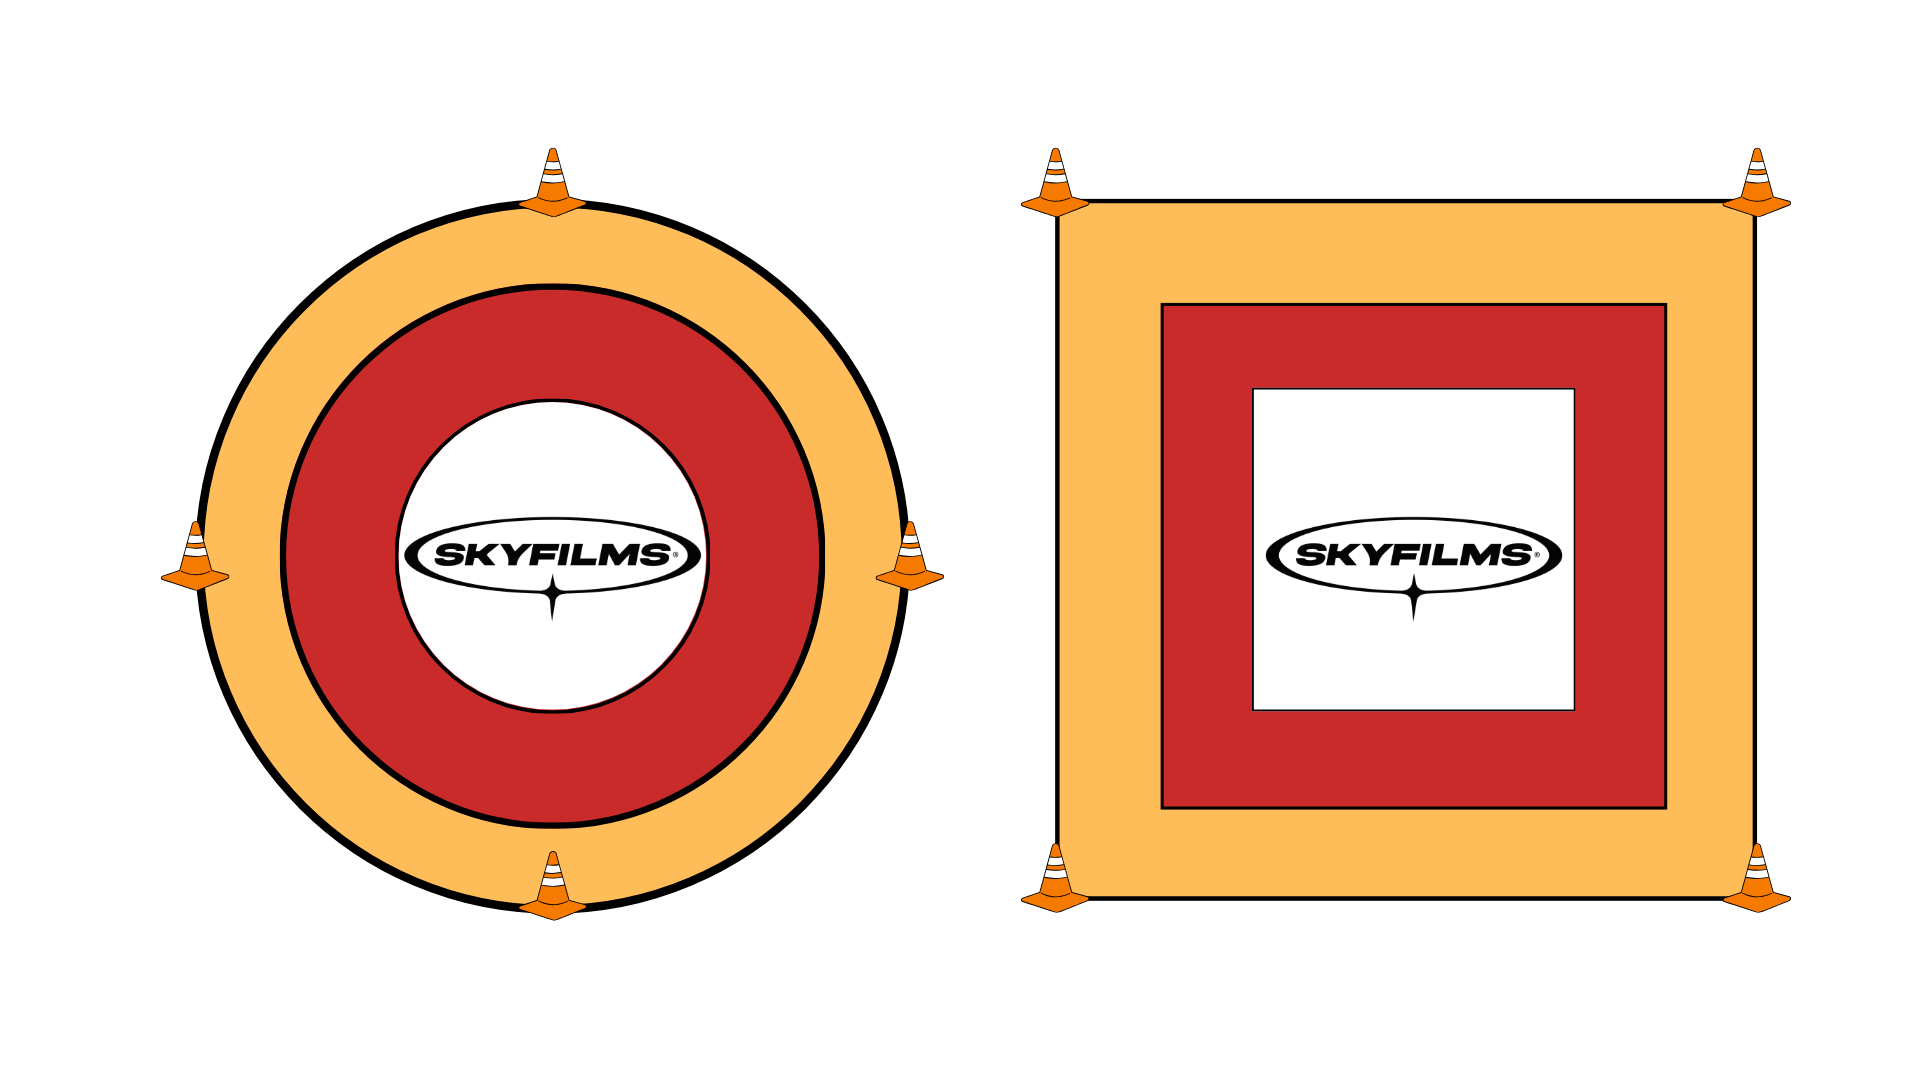
\includegraphics[width=.82\textwidth]{Imagenes/IMG_1597.PNG}
\caption{Ejemplo de delimitación física de un Área de Operación Temporal mediante conos y cinta de seguridad.}
\label{fig:delimitacion}
\end{figure}


\begin{figure}[H]
\centering
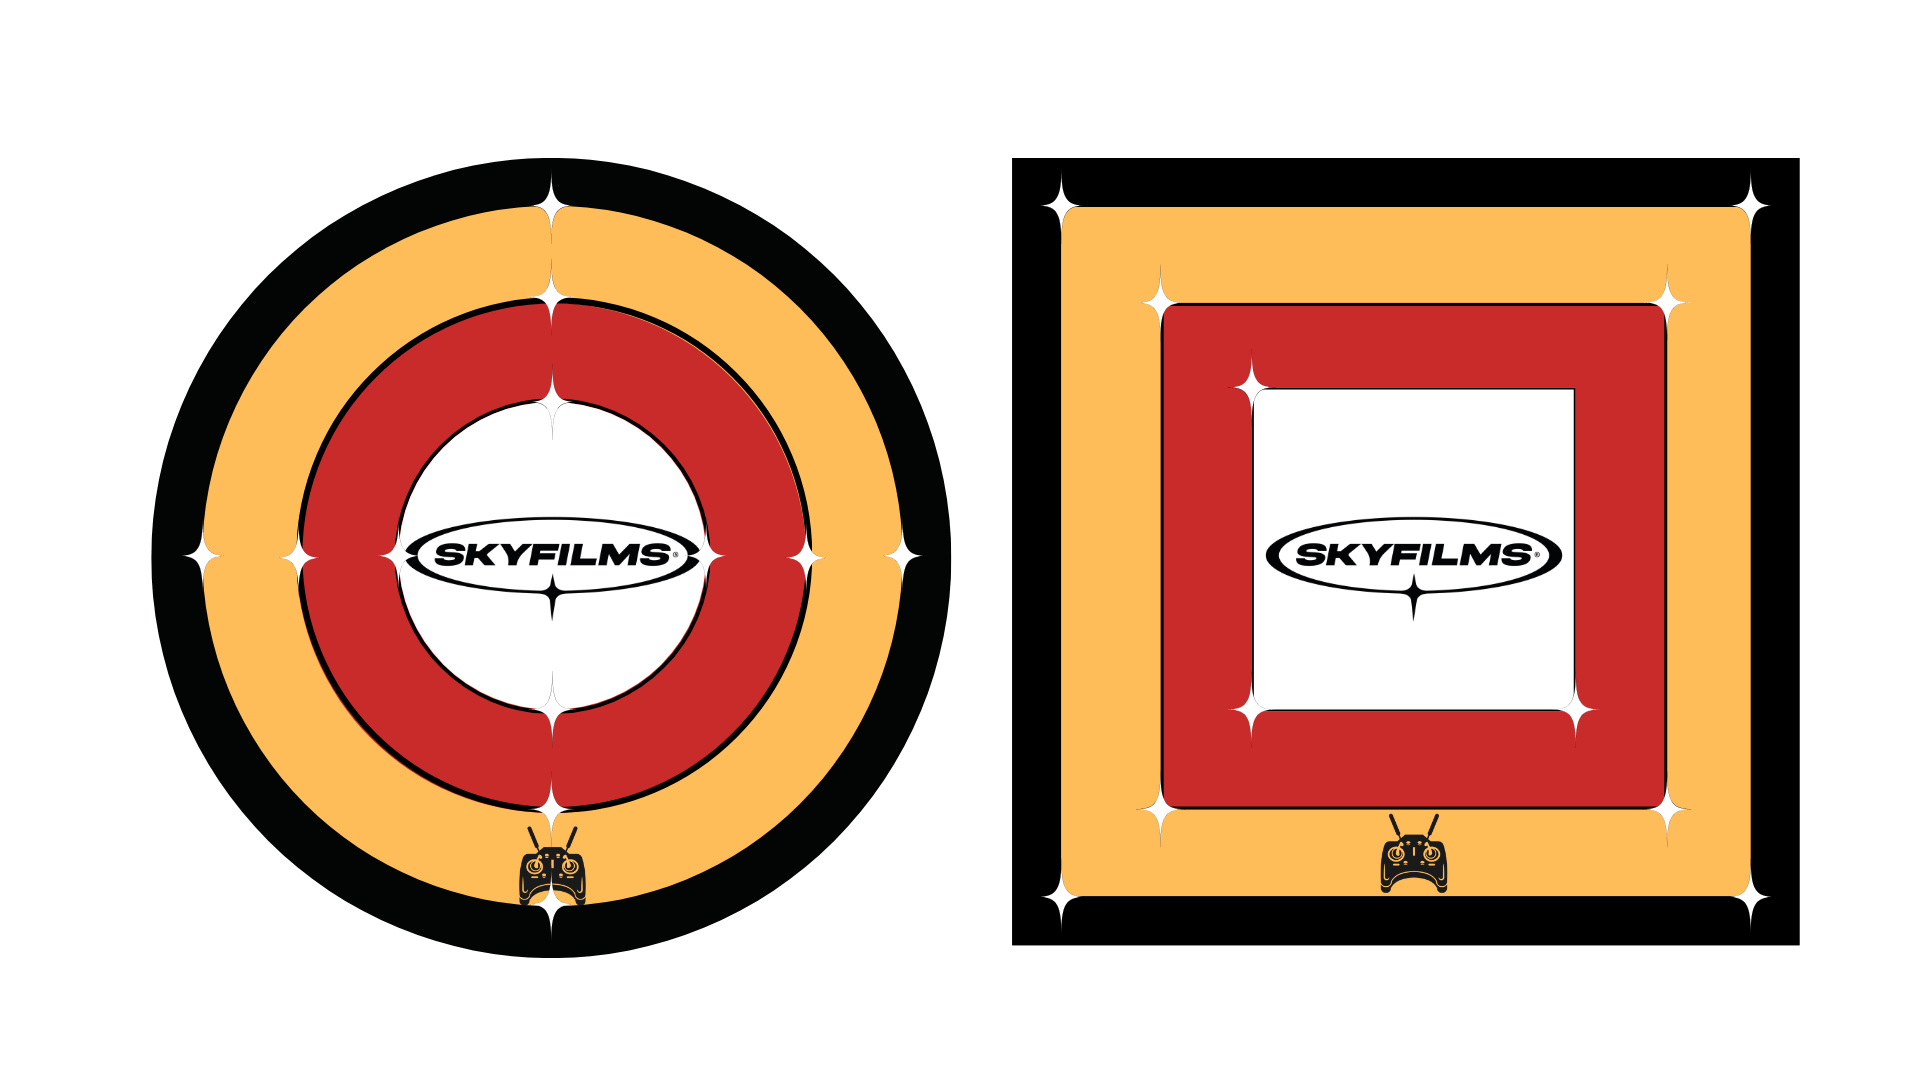
\includegraphics[width=.75\textwidth]{Imagenes/IMG_1596.PNG}
\caption{Ejemplo de iluminación portátil para operaciones en condiciones de baja iluminación.}
\label{fig:iluminacion}
\end{figure}


\begin{tcolorbox}[title=Documentos asociados,colback=gray!5,colframe=black]

\textbf{Procedimiento relacionado}

PO-001 – Planificación de la Operación

\vspace{0.3cm}

\textbf{Formatos relacionados}

\begin{itemize}

\item F-009 – Planificación de la Operación

\item F-011 – Evaluación del Riesgo Operacional

\item F-002 – Lista de Chequeo Preoperacional

\item F-010 – Briefing Operacional

\end{itemize}

\end{tcolorbox}







\subsection{Criterios para cancelar o reprogramar una operación}

Una operación deberá cancelarse, suspenderse o reprogramarse cuando se presente alguna de las siguientes condiciones:

\begin{itemize}

\item Condiciones meteorológicas incompatibles con una operación segura.

\item Restricciones del espacio aéreo que impidan la realización de la misión.

\item Fallas técnicas del UAS o de cualquiera de sus sistemas.

\item Indisponibilidad de personal competente.

\item Riesgos operacionales que superen el nivel aceptable definido por Skyfilms.

\item Ausencia de permisos o autorizaciones requeridas.

\item Cualquier otra condición que comprometa la seguridad operacional.

\end{itemize}

\begin{tcolorbox}[title=Documentos asociados,colback=gray!5,colframe=black]

\textbf{Procedimiento relacionado}

SOP-001 Planificación de la Operación.

\vspace{0.2cm}

\textbf{Formatos relacionados}

\begin{itemize}
\item F-008 Solicitud de Servicio.
\item F-009 Planificación de la Operación.
\item F-002 Lista de Chequeo Preoperacional.
\item F-001 Libro de Vuelo.
\end{itemize}

\end{tcolorbox}





\section{Evaluación del riesgo operacional}

Antes de la ejecución de cualquier operación UAS, Skyfilms S.A.S. realizará una evaluación del riesgo operacional con el fin de identificar los peligros asociados a la misión, analizar el nivel de riesgo y establecer las medidas de mitigación necesarias para garantizar un nivel de seguridad aceptable.

La evaluación del riesgo forma parte del proceso de planificación de la operación y constituye un requisito obligatorio antes de autorizar el inicio de cualquier misión.


\subsection{Objetivo}

La evaluación del riesgo operacional tiene como finalidad:

\begin{itemize}

\item Identificar peligros antes del inicio de la operación.

\item Analizar las amenazas presentes en el entorno operacional.

\item Definir medidas de mitigación.

\item Determinar la viabilidad operacional de la misión.

\item Proteger a las personas, bienes, espacio aéreo y aeronaves.

\end{itemize}

\subsection{Factores mínimos de evaluación}

\renewcommand{\arraystretch}{1.3}

\begin{longtable}{|p{5cm}|p{9cm}|}

\hline

\textbf{Factor} &
\textbf{Aspectos a evaluar}

\\ \hline

Espacio aéreo &
Clasificación, restricciones, NOTAM y proximidad a aeródromos.

\\ \hline

Meteorología &
Viento, lluvia, visibilidad, nubosidad y temperatura.

\\ \hline

Terreno &
Obstáculos, edificaciones, líneas eléctricas, cuerpos de agua y vegetación.

\\ \hline

Personas &
Presencia de terceros y control del área de operación.

\\ \hline

Infraestructura &
Edificaciones críticas, antenas, vías, puentes y otras estructuras.

\\ \hline

Tripulación &
Competencia, experiencia, estado físico y condición psicofísica.

\\ \hline

Aeronave &
Disponibilidad técnica, mantenimiento y estado general.

\\ \hline

Baterías &
Nivel de carga, ciclos, temperatura y estado físico.

\\ \hline

\end{longtable}

\subsection{Clasificación del riesgo}

Los riesgos identificados durante la planificación serán clasificados conforme a la metodología establecida en el Sistema de Gestión de la Seguridad Operacional (SMS).

Como criterio general, Skyfilms utilizará tres niveles de clasificación:

\begin{itemize}

\item Riesgo Bajo.

\item Riesgo Medio.

\item Riesgo Alto.

\end{itemize}

Las operaciones clasificadas como riesgo alto únicamente podrán ejecutarse cuando las medidas de mitigación implementadas permitan reducir el riesgo a un nivel aceptable.

\subsection{Medidas de mitigación}

Cuando durante la evaluación se identifique un riesgo operacional, podrán implementarse, entre otras, las siguientes medidas:

\begin{itemize}

\item Modificar el horario de la operación.

\item Cambiar el punto de despegue.

\item Reducir la altura de vuelo.

\item Delimitar el área de seguridad.

\item Incorporar un Observador Visual adicional.

\item Utilizar una aeronave diferente.

\item Posponer la misión.

\item Cancelar la operación.

\end{itemize}


\subsection{Aprobación}

La operación únicamente podrá iniciarse cuando la evaluación del riesgo haya sido completada y el nivel de riesgo residual resulte aceptable conforme a los criterios establecidos por Skyfilms.

Cuando el riesgo residual permanezca por encima del nivel aceptable, la misión deberá ser cancelada o reprogramada.



\begin{tcolorbox}[title=Documentos asociados,colback=gray!5,colframe=black]

\textbf{Procedimiento relacionado}

PO-002 Evaluación del Riesgo Operacional.

\vspace{0.2cm}

\textbf{Formatos relacionados}

\begin{itemize}

\item F-011 Evaluación del Riesgo Operacional.

\item F-009 Planificación de la Operación.

\item F-006 Reporte SMS (cuando aplique).

\end{itemize}

\end{tcolorbox}


\section{Briefing Operacional}

Antes del inicio de cualquier operación UAS, la tripulación deberá realizar un briefing operacional con el propósito de verificar que todas las condiciones técnicas, operacionales y de seguridad requeridas para la misión han sido comprendidas por el personal involucrado.

El briefing constituye la última verificación antes del inicio de la operación y permitirá confirmar que la planificación aprobada continúa siendo válida para las condiciones existentes en el lugar de la operación.

\subsection{Objetivos}

El briefing operacional tiene como objetivos:

\begin{itemize}

\item Confirmar el objetivo de la misión.

\item Asignar funciones y responsabilidades.

\item Revisar las condiciones meteorológicas reales.

\item Confirmar la disponibilidad técnica de la aeronave.

\item Revisar la evaluación del riesgo.

\item Verificar los procedimientos normales y de emergencia.

\item Resolver dudas antes del inicio de la operación.

\end{itemize}


\subsection{Participantes}

El briefing deberá realizarse con la participación de todo el personal involucrado en la operación, incluyendo, cuando aplique:

\begin{itemize}

\item Jefe de Pilotos.

\item Piloto Remoto.

\item Observador Visual.

\item Personal de apoyo.

\item Cliente o representante del cliente (cuando sea pertinente).

\end{itemize}

\subsection{Contenido mínimo}

\renewcommand{\arraystretch}{1.3}

\begin{longtable}{|p{5cm}|p{9cm}|}

\hline

\textbf{Tema} &
\textbf{Aspectos a revisar}

\\ \hline

Objetivo de la misión &
Alcance del servicio y producto esperado.

\\ \hline

Área de operación &
Zona de vuelo, límites, obstáculos y puntos de referencia.

\\ \hline

Meteorología &
Condiciones observadas antes del vuelo.

\\ \hline

Tripulación &
Asignación de funciones.

\\ \hline

Aeronave &
Estado técnico y configuración.

\\ \hline

Comunicaciones &
Canales de comunicación y palabras clave.

\\ \hline

Emergencias &
Procedimientos aplicables y puntos de reunión.

\\ \hline

Zonas de seguridad &
Despegue, aterrizaje y áreas restringidas.

\\ \hline

Terceros &
Control de acceso y protección de personas.

\\ \hline

\end{longtable}


\subsection{Confirmación de la tripulación}

Antes del inicio de la operación, el Piloto Remoto confirmará verbalmente que:

\begin{itemize}

\item La misión ha sido comprendida.

\item La aeronave se encuentra disponible para la operación.

\item Se conocen los procedimientos de emergencia.

\item No existen condiciones que impidan la ejecución segura de la misión.

\end{itemize}

El Observador Visual confirmará igualmente que comprende sus funciones y mantendrá comunicación permanente con el Piloto Remoto durante toda la operación.

\subsection{Modificaciones de última hora}

Cuando durante el briefing se identifiquen cambios significativos respecto a la planificación inicial, el Jefe de Pilotos deberá determinar si:

\begin{itemize}

\item La operación puede continuar sin modificaciones.

\item Es necesario actualizar la planificación.

\item Debe realizarse una nueva evaluación del riesgo.

\item La misión debe ser suspendida o reprogramada.

\end{itemize}


\begin{tcolorbox}[title=Documentos asociados,colback=gray!5,colframe=black]

\textbf{Procedimiento relacionado}

PO-003 Briefing Operacional.

\vspace{0.2cm}

\textbf{Formatos relacionados}

\begin{itemize}

\item F-010 Briefing Operacional.

\item F-009 Planificación de la Operación.

\item F-011 Evaluación del Riesgo Operacional.

\item F-002 Lista de Chequeo Preoperacional.

\end{itemize}

\end{tcolorbox}

\section{Ejecución de la Operación}

La ejecución de una operación UAS comprende el conjunto de actividades desarrolladas desde el inicio de la inspección preoperacional hasta la finalización del vuelo y aseguramiento de la aeronave.

Todas las operaciones deberán ejecutarse conforme a la planificación aprobada, la evaluación del riesgo realizada, las limitaciones establecidas en las OpSpecs y los procedimientos definidos en el presente Manual de Operaciones.









\subsection{Inspección preoperacional}

Antes de cada vuelo, el Piloto Remoto deberá realizar una inspección preoperacional de la aeronave y de todos los equipos asociados.

La inspección tendrá como finalidad verificar que la aeronave se encuentra en condiciones técnicas adecuadas para la operación y que no existen condiciones que comprometan la seguridad del vuelo.

La inspección deberá quedar registrada mediante la Lista de Chequeo Preoperacional correspondiente.


\subsubsection*{Aspectos mínimos a verificar}

\begin{itemize}

\item Estado general de la aeronave.

\item Integridad estructural.

\item Hélices correctamente instaladas.

\item Estado de motores.

\item Nivel de carga de baterías.

\item Estado del control remoto.

\item Sistema de navegación.

\item Sistema de posicionamiento.

\item Tarjeta de memoria.

\item Configuración de Return To Home (RTH).

\item Espacio aéreo habilitado.

\item Área libre para despegue y aterrizaje.

\end{itemize}


\subsection{Inicio de la operación}

Antes del despegue, el Piloto Remoto verificará que:

\begin{itemize}

\item El briefing haya finalizado.

\item La evaluación del riesgo se encuentre aprobada.

\item No existan cambios significativos en las condiciones meteorológicas.

\item El área de operación permanezca controlada.

\item El Observador Visual se encuentre en posición.

\item La aeronave disponga de suficiente autonomía para cumplir la misión.

\end{itemize}

Únicamente cuando todas estas condiciones hayan sido verificadas podrá iniciarse el vuelo.


\subsection{Desarrollo del vuelo}

Durante la ejecución de la misión, el Piloto Remoto deberá:

\begin{enumerate}

\item Mantener el control de la aeronave en todo momento.

\item Operar dentro de las limitaciones autorizadas.

\item Supervisar permanentemente el estado del UAS.

\item Mantener comunicación con el Observador Visual cuando aplique.

\item Monitorear continuamente el entorno operacional.

\item Interrumpir inmediatamente la operación cuando se identifique una condición insegura.

\end{enumerate}

\subsection{Funciones del Observador Visual durante la operación}

Cuando la operación requiera Observador Visual, este deberá:

\begin{itemize}

\item Mantener contacto visual permanente con la aeronave.

\item Informar oportunamente cualquier riesgo.

\item Vigilar la presencia de terceros.

\item Alertar sobre otras aeronaves.

\item Supervisar el área de seguridad.

\item Apoyar la aplicación de procedimientos de emergencia.

\end{itemize}


\subsection{Suspensión inmediata de la operación}

El Piloto Remoto deberá suspender inmediatamente la operación cuando ocurra cualquiera de las siguientes situaciones:

\begin{itemize}

\item Pérdida de control de la aeronave.

\item Aparición de aeronaves tripuladas.

\item Ingreso de personas al área crítica de operación.

\item Condiciones meteorológicas adversas.

\item Advertencias críticas del sistema.

\item Disminución del nivel de batería por debajo de los límites establecidos.

\item Cualquier condición que comprometa la seguridad operacional.

\end{itemize}

\subsection{Finalización del vuelo}

Una vez concluida la misión, el Piloto Remoto deberá:

\begin{enumerate}

\item Aterrizar en la zona prevista.

\item Apagar la aeronave.

\item Asegurar las baterías.

\item Realizar una inspección visual posterior al vuelo.

\item Informar cualquier novedad presentada durante la operación.

\item Registrar la información correspondiente en el Libro de Vuelo.

\end{enumerate}

\begin{tcolorbox}[title=Documentos asociados,colback=gray!5,colframe=black]

\textbf{Procedimiento relacionado}

PO-004 Ejecución de la Operación.

\vspace{0.3cm}

\textbf{Formatos relacionados}

\begin{itemize}

\item F-001 Libro de Vuelo.

\item F-002 Lista de Chequeo Preoperacional.

\item F-003 Lista de Chequeo Postoperacional.

\item F-009 Planificación de la Operación.

\item F-010 Briefing Operacional.

\item F-011 Evaluación del Riesgo Operacional.

\end{itemize}

\end{tcolorbox}

\section{Gestión del Enlace (C2)}

El enlace de Mando y Control (Command and Control - C2) constituye el medio principal de comunicación entre la estación de control en tierra y la aeronave no tripulada, permitiendo la transmisión de comandos, telemetría y demás información necesaria para el desarrollo seguro de la operación.

Durante todas las fases del vuelo, el Piloto Remoto será responsable de supervisar permanentemente la calidad del enlace C2 y de adoptar las acciones necesarias cuando se presenten degradaciones o pérdidas del mismo.

Skyfilms utilizará sistemas de enlace C2 certificados por los fabricantes de las aeronaves empleadas, configurados conforme a las recomendaciones técnicas y a las limitaciones establecidas por la normativa aplicable.


\subsection{Supervisión del enlace C2}

Antes y durante cada operación, el Piloto Remoto deberá verificar continuamente el estado del enlace C2 mediante los indicadores disponibles en la estación de control.

Como mínimo deberán supervisarse los siguientes parámetros:

\renewcommand{\arraystretch}{1.3}

\begin{longtable}{|p{4.5cm}|p{4cm}|p{4cm}|}
\hline

\textbf{Parámetro} &
\textbf{DJI Mavic 4 Pro} &
\textbf{Pavo20 Pro}

\\ \hline

Calidad del enlace &
Indicador de señal &
RSSI / LQ

\\ \hline

Telemetría &
Disponible &
Disponible

\\ \hline

Alertas visuales &
Sí &
Sí

\\ \hline

Alertas sonoras &
Sí &
Sí

\\ \hline

Estado del enlace &
En tiempo real &
En tiempo real

\\ \hline

\end{longtable}



\subsection{Gestión de la degradación del enlace}

Cuando durante la operación se detecte una disminución en la calidad del enlace C2, el Piloto Remoto deberá adoptar, según corresponda, las siguientes acciones:

\begin{itemize}

\item Reducir la distancia respecto a la aeronave.

\item Disminuir la altura de operación cuando resulte conveniente.

\item Reorientar las antenas del sistema de control.

\item Evitar obstáculos que puedan afectar la propagación de la señal.

\item Mantener comunicación permanente con el Observador Visual.

\item Prepararse para finalizar la misión si la condición persiste.

\end{itemize}

\begin{figure}[H]
\centering
\begin{tikzpicture}[
font=\small,
node distance=7mm,
box/.style={
rectangle,
rounded corners,
draw,
align=center,
minimum width=4.5cm,
minimum height=0.9cm
},
arrow/.style={
-{Latex},
thick
}
]

\node[box] (a) {Operación normal};

\node[box, below=of a] (b) {Degradación del enlace C2};

\node[box, below=of b] (c) {Aplicar medidas correctivas};

\node[box, below=of c] (d) {¿Se recupera el enlace?};

\node[box, below left=1cm and 1.8cm of d] (e) {Continuar la operación};

\node[box, below right=1cm and 1.8cm of d] (f) {Activar procedimiento de pérdida del enlace};

\node[box, below=of f] (g) {RTH / LAND / Failsafe};

\node[box, below=of g] (h) {Registrar evento e informar al SMS};

\draw[arrow] (a)--(b);
\draw[arrow] (b)--(c);
\draw[arrow] (c)--(d);

\draw[arrow] (d)--node[left]{Sí}(e);
\draw[arrow] (d)--node[right]{No}(f);

\draw[arrow] (f)--(g);
\draw[arrow] (g)--(h);

\end{tikzpicture}

\caption{Gestión general de la degradación del enlace C2.}
\end{figure}


\subsection{Pérdida del enlace C2}

Cuando se presente una pérdida total del enlace de mando y control, la tripulación deberá aplicar los procedimientos automáticos y operacionales definidos para cada tipo de aeronave.

\renewcommand{\arraystretch}{1.3}

\begin{longtable}{|p{4.5cm}|p{6cm}|p{3cm}|}

\hline

\textbf{Sistema} &
\textbf{Acción inmediata} &
\textbf{Continuidad}

\\ \hline

DJI Mavic 4 Pro &
Permitir la activación automática del Return To Home (RTH) o del procedimiento configurado para pérdida de enlace. &
Cancelar la misión.

\\ \hline

Pavo20 Pro &
Permitir la ejecución del Failsafe configurado (RTH, LAND o procedimiento autorizado). &
Cancelar la misión.

\\ \hline

\end{longtable}


\subsection{Gestión de interferencias}

Cuando se identifique una posible interferencia electromagnética que afecte el enlace C2, el Piloto Remoto deberá:

\begin{itemize}

\item Identificar el origen probable de la interferencia.

\item Modificar la posición de operación cuando sea posible.

\item Evitar la proximidad a fuentes conocidas de interferencia.

\item Suspender la operación cuando no sea posible garantizar un enlace seguro.

\end{itemize}

Las interferencias podrán originarse por:

\begin{itemize}

\item Redes Wi-Fi.

\item Infraestructura de telecomunicaciones.

\item Equipos industriales.

\item Condiciones atmosféricas.

\item Obstáculos físicos.

\end{itemize}


\subsection{Limitaciones operacionales}

La confiabilidad del enlace C2 dependerá de factores propios del entorno operacional y de las características técnicas del sistema empleado.

Durante las operaciones deberán considerarse, entre otras, las siguientes limitaciones:

\begin{itemize}

\item Obstáculos naturales o artificiales.

\item Condiciones meteorológicas adversas.

\item Interferencias electromagnéticas.

\item Tipo de operación autorizada (VLOS).

\item Distancia entre la estación de control y la aeronave.

\end{itemize}

\subsection{Referencias técnicas}

Las especificaciones técnicas particulares de cada sistema de enlace C2, incluyendo frecuencias de operación, protocolos de comunicación, configuraciones de \textit{failsafe}, firmware, equipos compatibles y demás características técnicas, se encuentran documentadas en las Fichas Técnicas de Aeronave (FTA) y en el Manual de Control de Mantenimiento (MCM), documentos controlados por Skyfilms S.A.S.

Las FTA forman parte del Sistema de Gestión Documental de la organización y deberán mantenerse actualizadas conforme a las configuraciones aprobadas para cada aeronave.

\begin{tcolorbox}[
title=Nota Operacional,
colback=blue!5,
colframe=blue!60!black]

El Piloto Remoto deberá considerar cualquier degradación del enlace C2 como una condición potencialmente insegura. Si las medidas de mitigación no restablecen un nivel aceptable de confiabilidad del enlace, la misión deberá finalizar de manera controlada y el evento será registrado conforme a los procedimientos del Sistema de Gestión de la Seguridad Operacional (SMS).

\end{tcolorbox}










\section{Procedimientos especiales de operación}

Determinadas operaciones desarrolladas por Skyfilms requieren la adopción de medidas adicionales de planificación, coordinación y control debido a las características particulares del entorno operacional o del tipo de misión.

Los procedimientos descritos en esta sección complementan los procedimientos generales establecidos en el presente Manual de Operaciones y deberán aplicarse cuando corresponda.


\subsection{Operaciones FPV}

Las operaciones mediante aeronaves FPV (\textit{First Person View}) estarán destinadas a la obtención de secuencias audiovisuales dinámicas y se ejecutarán estrictamente bajo condiciones de Visibilidad en Línea de Vista (VLOS), conforme a lo establecido en el RAC 100.

Dado que el Piloto Remoto utiliza un dispositivo de visión en primera persona (gafas/visor) que limita su percepción visual del entorno circundante, es de carácter \textbf{obligatorio} el cumplimiento de las siguientes directrices operacionales para mitigar el riesgo:

\begin{itemize}
    \item \textbf{Observador Visual Dedicado:} Toda operación FPV debe contar obligatoriamente con la presencia ininterrumpida de al menos un Observador Visual.
    \item \textbf{Contacto Visual Directo (VLOS):} El Observador Visual será el responsable de mantener el contacto visual directo y constante con la aeronave (UA) y su entorno en todo momento, sin el uso de ayudas ópticas o electrónicas (diferentes a lentes correctivos).
    \item \textbf{Comunicación Efectiva:} Debe existir una comunicación verbal clara, constante y en tiempo real entre el Piloto Remoto y el Observador Visual para alertar sobre obstáculos, tráfico aéreo tripulado o incursiones de terceros.
    \item \textbf{Límites del Área de Operación:} El área de vuelo debe ser evaluada previamente para garantizar que la aeronave nunca exceda el radio visual del Observador (límite máximo legal de 750 metros horizontales).
\end{itemize}<


\subsection{Operaciones en zonas urbanas}

Antes de operar en entornos urbanos deberá verificarse:

\begin{itemize}

\item Presencia de terceros.

\item Obstáculos verticales.

\item Interferencias electromagnéticas.

\item Disponibilidad de zonas de aterrizaje de emergencia.

\item Control del perímetro operacional.

\end{itemize}

\subsection{Operaciones cerca de infraestructura}

Cuando la operación se realice en proximidad de edificaciones, puentes, torres, antenas u otras estructuras, el Piloto Remoto deberá:

\begin{enumerate}

\item Mantener una distancia de seguridad.

\item Identificar posibles efectos de turbulencia.

\item Verificar la recepción GNSS.

\item Mantener rutas de escape previamente definidas.

\end{enumerate}


\subsection{Operaciones en eventos}

Las operaciones destinadas al cubrimiento de eventos deberán considerar, como mínimo:

\begin{itemize}

\item Control del público.

\item Coordinación con el organizador.

\item Delimitación del área de operación.

\item Identificación de rutas de evacuación.

\item Procedimientos para suspensión inmediata del vuelo.

\end{itemize}

Cuando la operación implique concentraciones de personas, únicamente podrá desarrollarse si cuenta con las autorizaciones exigidas por la Aeronáutica Civil y se han implementado las medidas de mitigación correspondientes.



\subsection{Operaciones en zonas rurales}

Durante operaciones en áreas rurales deberán evaluarse, entre otros:

\begin{itemize}

\item Líneas eléctricas.

\item Árboles.

\item Animales.

\item Condiciones del terreno.

\item Cobertura de comunicaciones.

\end{itemize}


\subsection{Operaciones cerca de cuerpos de agua}

Cuando la misión se desarrolle sobre o cerca de cuerpos de agua, deberán adoptarse medidas adicionales para:

\begin{itemize}

\item Identificar zonas seguras de aterrizaje.

\item Evitar pérdida de referencia visual.

\item Considerar efectos del viento.

\item Establecer procedimientos ante amerizaje accidental.

\end{itemize}


\subsection{Vuelo Nocturno}

Skyfilms S.A.S. ejecutará operaciones de vuelo nocturno para la captura de material audiovisual cinematográfico y comercial, dando estricto cumplimiento a las exigencias operacionales y de seguridad establecidas por la Aerocivil para la Categoría Específica.

Para la ejecución y autorización de vuelos nocturnos, el Piloto Remoto y el equipo operativo deberán verificar y cumplir ineludiblemente con los siguientes requisitos previos y durante el vuelo:

\begin{itemize}
    \item \textbf{Adición en el Certificado:} El Piloto Remoto al mando debe contar de manera obligatoria con la adición vigente de ``Vuelo Nocturno'' en su Certificado de Idoneidad como piloto UAS (CIPU).
    \item \textbf{Iluminación de la Aeronave:} La aeronave no tripulada (UA) debe operar con las luces instaladas de fábrica o autorizadas por su fabricante, encendidas de forma permanente durante toda la operación nocturna (RAC 100.220 a). Estas luces deben hacer a la aeronave claramente visible en el cielo nocturno para la tripulación y para otras aeronaves en el espacio aéreo. En el DJI Mavic 4 Pro, los ledes delanteros se configuran para permanecer encendidos; el modo \textit{Auto} los apaga al grabar y no debe usarse de noche. Antes de cada vuelo se verifica que las luces funcionan, y no se instalan accesorios que no estén autorizados por el fabricante.
    \item \textbf{Modalidad de Vuelo Estricta:} La operación nocturna se restringirá \textbf{únicamente a la modalidad VLOS} (Visibilidad en Línea de Vista), sin exceder en ningún momento un radio de 750 metros horizontales medidos desde la posición fija del piloto.
    \item \textbf{Reconocimiento Diurno Obligatorio (Scouting):} Es de carácter mandatorio realizar una inspección física y visual del área de operación en horario diurno (con luz solar) antes de la ejecución del vuelo nocturno en esa misma locación. Este reconocimiento tiene como objetivo principal la identificación de obstáculos no iluminados (líneas eléctricas, cables, antenas, vegetación alta) y el establecimiento de rutas de vuelo seguras y puntos de aterrizaje de emergencia.
    \item \textbf{Apoyo de Observador Visual:} Toda operación nocturna requerirá incondicionalmente el apoyo de un Observador Visual asignado por el Jefe de Pilotos, quien asistirá en el monitoreo del entorno para prevenir colisiones e identificar cualquier amenaza en la oscuridad.
    \item \textbf{Límites de la operación:} el tiempo de vuelo planificado no excederá el 80\,\% de la autonomía de la aeronave (RAC 100.210 k); la operación se realiza desde un punto fijo (RAC 100.210 n) y a una altura máxima de 400 ft (122 m) sobre el terreno. En zona urbana se mantiene una distancia mínima de 30 m a personas y edificaciones (RAC 100.220 b).
    \item \textbf{Falla de iluminación:} si las luces de la aeronave se apagan o fallan durante el vuelo, el Piloto Remoto aterriza de inmediato en el punto seguro más cercano e informa al Observador Visual y al Jefe de Pilotos.
    \item \textbf{Lista de chequeo y riesgo nocturno:} toda operación nocturna incluye la sección nocturna de la Lista de Chequeo Preoperacional (F-002) y una Evaluación del Riesgo Operacional (F-011) que considere la pérdida de referencias visuales, la desorientación espacial y los obstáculos no iluminados.
\end{itemize}

\section{Procedimientos Anormales y de Emergencia}

Skyfilms S.A.S. establece procedimientos estandarizados para responder de manera rápida, segura y coordinada ante condiciones anormales o situaciones de emergencia que puedan presentarse durante las operaciones UAS.

El objetivo de estos procedimientos es proteger la vida e integridad de las personas, preservar la seguridad del espacio aéreo, minimizar daños materiales y garantizar la adecuada gestión posterior del evento.


\subsection{Generalidades}

Ante cualquier condición anormal o emergencia, el Piloto Remoto deberá aplicar los siguientes principios:

\begin{enumerate}

\item Mantener la calma.

\item Priorizar la seguridad de las personas.

\item Mantener el control de la aeronave cuando sea posible.

\item Aplicar el procedimiento correspondiente.

\item Informar inmediatamente al Observador Visual.

\item Suspender la operación cuando la seguridad operacional se vea comprometida.

\item Reportar el evento conforme al Sistema de Gestión de la Seguridad Operacional (SMS).

\end{enumerate}

\subsection{Clasificación de condiciones anormales y emergencias}

Las situaciones que puedan presentarse durante una operación UAS se clasifican en las siguientes categorías:

\begin{enumerate}[label=\Alph*.]

\item Condiciones Anormales

\item Emergencias Técnicas

\item Emergencias Operacionales

\item Emergencias Ambientales

\item Emergencias Médicas

\item Accidentes

\end{enumerate}


\subsection{Condiciones Anormales}

Se consideran condiciones anormales aquellas situaciones que afectan el desarrollo de la misión, pero que permiten mantener el control de la aeronave y finalizar la operación de manera segura mediante la aplicación de los procedimientos establecidos.

\renewcommand{\arraystretch}{1.4}

\begin{longtable}{|p{4.5cm}|p{6cm}|p{3.5cm}|}
\hline

\textbf{Condición} &
\textbf{Acción inmediata} &
\textbf{Continuidad}

\\ \hline

Incremento del viento &
Evaluar la estabilidad del vuelo y considerar el retorno al punto de aterrizaje. &
Continuar únicamente si el riesgo permanece aceptable.

\\ \hline

Disminución de señal GNSS &
Mantener el control manual, evitar maniobras críticas y monitorear la estabilidad de la aeronave. &
Reevaluar la misión.

\\ \hline

Consumo elevado de batería &
Reducir la duración de la misión y regresar de inmediato al punto de aterrizaje. &
Finalizar la operación.

\\ \hline

Pérdida temporal del video FPV &
Mantener comunicación con el Observador Visual y recuperar el enlace de video. &
Continuar únicamente si el enlace se restablece completamente.

\\ \hline

\end{longtable}




\subsection{Emergencias Técnicas}

Las emergencias técnicas corresponden a fallas del sistema UAS que pueden comprometer la seguridad de la operación y requieren una respuesta inmediata.

\renewcommand{\arraystretch}{1.4}

\begin{longtable}{|p{4.5cm}|p{6cm}|p{3.5cm}|}
\hline

\textbf{Emergencia} &
\textbf{Acción inmediata} &
\textbf{Continuidad}

\\ \hline

Pérdida del enlace C2 &
Esperar la recuperación automática del enlace o la activación del Return To Home (RTH). &
Cancelar la misión.

\\ \hline

Fly Away &
Intentar recuperar el control, alertar al Observador Visual y proteger a terceros. &
Operación suspendida.

\\ \hline

Falla de motor &
Realizar aterrizaje inmediato en una zona segura. &
Operación suspendida.

\\ \hline

Falla de hélice &
Reducir riesgos para terceros y aterrizar inmediatamente. &
Operación suspendida.

\\ \hline

Error crítico del sistema &
Suspender la operación y asegurar la aeronave. &
Operación suspendida.

\\ \hline

\end{longtable}


\subsection{Emergencias Operacionales}

Las emergencias operacionales corresponden a situaciones originadas por factores externos durante el desarrollo de la misión.

\renewcommand{\arraystretch}{1.4}

\begin{longtable}{|p{4.5cm}|p{6cm}|p{3.5cm}|}
\hline

\textbf{Emergencia} &
\textbf{Acción inmediata} &
\textbf{Continuidad}

\\ \hline

Ingreso de personas al área &
Suspender temporalmente la operación y mantener la aeronave en condición segura o aterrizar si es necesario. &
Continuar únicamente cuando el área vuelva a estar controlada.

\\ \hline

Presencia de aeronave tripulada &
Descender inmediatamente o aterrizar, manteniendo separación segura. &
Reanudar únicamente cuando desaparezca el conflicto.

\\ \hline

Pérdida del Observador Visual &
Suspender inmediatamente la misión FPV y aterrizar la aeronave. &
Operación suspendida.

\\ \hline

Interferencia operacional &
Alejar la aeronave y reevaluar el escenario operacional. &
Continuar únicamente si desaparece la condición de riesgo.

\\ \hline

\end{longtable}

\subsection{Emergencias Ambientales}

Las emergencias ambientales corresponden a cambios inesperados en las condiciones del entorno.

\renewcommand{\arraystretch}{1.4}

\begin{longtable}{|p{4.5cm}|p{6cm}|p{3.5cm}|}
\hline

\textbf{Emergencia} &
\textbf{Acción inmediata} &
\textbf{Continuidad}

\\ \hline

Lluvia &
Aterrizar inmediatamente. &
Cancelar la misión.

\\ \hline

Tormenta eléctrica &
Cancelar inmediatamente la operación y asegurar los equipos. &
Operación suspendida.

\\ \hline

Incremento súbito del viento &
Regresar al punto de aterrizaje. &
Reevaluar condiciones antes de continuar.

\\ \hline

Humo o incendio cercano &
Alejar la aeronave y abandonar el área afectada. &
Operación suspendida.

\\ \hline

Reducción significativa de la visibilidad &
Aterrizar tan pronto como sea seguro hacerlo. &
Cancelar la misión.

\\ \hline

\end{longtable}

\subsection{Emergencias Médicas}

Cuando durante una operación se presente una emergencia médica deberán aplicarse las siguientes acciones iniciales.

\renewcommand{\arraystretch}{1.4}

\begin{longtable}{|p{4.5cm}|p{6cm}|p{3.5cm}|}
\hline

\textbf{Emergencia} &
\textbf{Acción inmediata} &
\textbf{Continuidad}

\\ \hline

Lesión leve &
Aplicar primeros auxilios y evaluar la condición del afectado. &
Continuar únicamente si no existe afectación para la seguridad.

\\ \hline

Lesión grave &
Activar el Sistema de Emergencias Médicas (SEM) y suspender la operación. &
Operación suspendida.

\\ \hline

Incapacidad del Piloto Remoto &
Asegurar la aeronave y solicitar asistencia médica. &
Operación suspendida.

\\ \hline

Emergencia médica de un tercero &
Priorizar la atención del afectado y coordinar con los servicios de emergencia. &
Operación suspendida hasta garantizar condiciones seguras.

\\ \hline

\end{longtable}




\subsection{Accidentes}

Cuando ocurra un accidente durante una operación UAS, la tripulación deberá:

\begin{enumerate}

\item Priorizar la atención de personas lesionadas.

\item Asegurar el área de operación.

\item Evitar modificar la escena del evento salvo que exista riesgo adicional.

\item Informar al Jefe de Pilotos.

\item Informar al Gerente SMS.

\item Preservar la evidencia disponible.

\item Elaborar el reporte correspondiente conforme al SMS.

\end{enumerate}


\begin{tcolorbox}[title=Documentos asociados,colback=gray!5,colframe=black]

\textbf{Procedimiento relacionado}

PO-005 Gestión de Condiciones Anormales y Emergencias.

\vspace{0.3cm}

\textbf{Formatos relacionados}

\begin{itemize}

\item F-006 Reporte SMS.

\item F-012 Reporte de Peligros.

\item F-013 Reporte de Incidente o Accidente.

\item F-001 Libro de Vuelo.

\end{itemize}

\end{tcolorbox}


\section{Finalización de la Operación}

La finalización de una operación comprende todas las actividades posteriores al aterrizaje de la aeronave, orientadas a garantizar el cierre seguro de la misión, la preservación de los equipos, la actualización de los registros operacionales y la disponibilidad de la aeronave para futuras operaciones.

Ninguna misión se considerará finalizada hasta completar la totalidad de las actividades de cierre descritas en el presente procedimiento.

\subsection{Aseguramiento de la aeronave}

Una vez concluido el vuelo, el Piloto Remoto deberá:

\begin{enumerate}

\item Apagar la aeronave.

\item Apagar el control remoto.

\item Retirar la batería.

\item Verificar la temperatura de las baterías.

\item Realizar una inspección visual del UAS.

\item Asegurar todos los equipos antes del transporte.

\end{enumerate}


\subsection{Inspección postoperacional}

Después de cada operación deberá realizarse una inspección visual de la aeronave con el propósito de identificar daños, desgaste o cualquier condición que pueda afectar la aeronavegabilidad del UAS.

Como mínimo deberán verificarse:

\begin{itemize}

\item Estado estructural.

\item Hélices.

\item Motores.

\item Cámara.

\item Gimbal.

\item Baterías.

\item Antenas.

\item Tornillería visible.

\item Estado general de limpieza.

\end{itemize}


\subsection{Gestión de baterías}

Finalizada la operación, las baterías deberán:

\begin{itemize}

\item Registrarse en el control de baterías.

\item Verificarse visualmente.

\item Almacenarse conforme a las recomendaciones del fabricante.

\item Retirarse del servicio cuando presenten daños o comportamientos anormales.

\end{itemize}

\subsection{Gestión del material capturado}

Terminada la operación, el material audiovisual deberá descargarse, verificarse y almacenarse conforme al procedimiento interno de gestión de la información.

La descarga del material deberá realizarse antes de reutilizar las tarjetas de memoria empleadas durante la misión.


\subsection{Debriefing operacional}

Cuando la complejidad de la misión lo amerite, la tripulación realizará un debriefing con el propósito de:

\begin{itemize}

\item Analizar el desarrollo de la operación.

\item Identificar oportunidades de mejora.

\item Registrar novedades.

\item Identificar peligros observados.

\item Retroalimentar futuros procedimientos.

\end{itemize}

\subsection{Cierre operacional}

Antes de dar por finalizada la misión deberá verificarse que:

\begin{itemize}

\item Se diligenció el Libro de Vuelo.

\item Se diligenciaron los formatos aplicables.

\item No existen novedades pendientes.

\item La aeronave quedó disponible para una nueva operación o fue remitida a mantenimiento.

\item Los reportes SMS fueron realizados cuando corresponda.

\end{itemize}


\begin{tcolorbox}[title=Documentos asociados,colback=gray!5,colframe=black]

\textbf{Procedimiento relacionado}

PO-006 Finalización de la Operación.

\vspace{0.3cm}

\textbf{Formatos relacionados}

\begin{itemize}

\item F-001 Libro de Vuelo.

\item F-003 Lista de Chequeo Postoperacional.

\item F-004 Registro de Baterías.

\item F-006 Reporte SMS.

\item F-013 Reporte de Incidente o Accidente (cuando aplique).

\end{itemize}

\end{tcolorbox}



\section{Manejo y Transporte de Mercancías Peligrosas (Baterías UAS)}

Aunque Skyfilms S.A.S. excluye el transporte comercial de mercancías peligrosas como carga útil, reconoce que las baterías de Litio-Polímero (LiPo) y Iones de Litio (Li-ion) utilizadas para propulsar las aeronaves (Mavic 4 Pro y FPV) y equipos de estación de tierra, son clasificadas legalmente como Mercancías Peligrosas (Clase 9 - Varios) bajo la normativa aeronáutica internacional y nacional.

Para garantizar la seguridad operacional, el personal deberá cumplir estrictamente el siguiente procedimiento para el control, manejo, transporte, almacenamiento y disposición final de las baterías:

\begin{enumerate}
    \item \textbf{Transporte Terrestre y Aéreo:}
    \begin{itemize}
        \item Las baterías nunca deben transportarse instaladas en la aeronave.
        \item Deben transportarse descargadas a un nivel de almacenamiento seguro (entre 30\% y 50\% de su capacidad).
        \item Es obligatorio el uso de bolsas ignífugas (\textit{LiPo Safe Bags}) o estuches rígidos individuales que aíslen los terminales para prevenir cortocircuitos.
        \item En caso de desplazamiento en vuelos comerciales (aerolíneas), las baterías deben llevarse exclusivamente en el equipaje de mano, con los terminales aislados con cinta no conductiva, cumpliendo los límites de Watt-hora (Wh) de la IATA.
    \end{itemize}

    \item \textbf{Carga y Descarga en Locación:}
    \begin{itemize}
        \item La carga de baterías en campo se realizará exclusivamente en áreas ventiladas, alejadas de materiales inflamables y exposición directa al sol.
        \item El Piloto nunca dejará desatendido un proceso de carga.
        \item Si una batería presenta un incremento inusual de temperatura durante la carga, el proceso se interrumpirá inmediatamente y se aislará la batería.
    \end{itemize}

    \item \textbf{Almacenamiento y Mantenimiento:}
    \begin{itemize}
        \item Las baterías se almacenarán en la base principal en gabinetes ventilados a temperatura ambiente (15°C a 25°C).
        \item Se debe inspeccionar visualmente cada batería antes de su uso para descartar hinchamiento (\textit{puffing}), perforaciones, o cables expuestos. Una batería con cualquiera de estas condiciones se declarará inoperativa.
    \end{itemize}

    \item \textbf{Disposición Final:}
    \begin{itemize}
        \item Las baterías declaradas inoperativas o que hayan cumplido su ciclo de vida útil (aprox. 200 ciclos) no serán desechadas en la basura común.
        \item Serán descargadas completamente (0V) mediante un descargador resistivo o sumergidas en solución salina (protocolo LiPo), y posteriormente entregadas a un gestor ambiental certificado para el manejo de Residuos de Aparatos Eléctricos y Electrónicos (RAEE).
    \end{itemize}
\end{enumerate}

















% Fin del Capítulo 3



